\section{Our Estimators}
\label{sec:layeredbsdf:ours}

We now describe our specific layered BSDF method,
by presenting our Monte-Carlo solutions to enable the three key operations needed to fully define a BSDF model:
sampling (\S\ref{subsec:ours_sample}), evaluation (\S\ref{subsec:ours_eval}) and pdf computation (\S\ref{subsec:ours_pdf}).
Sampling produces the outgoing direction $\omegaout$ given the incoming one $\omegain$ (or the reverse), while evaluation answers the BSDF query for given $\omegain$ and $\omegaout$. Note that the values returned from sampling, evaluation and pdf procedures are themselves stochastic, and are equal to the true BSDF value, pdf value or sampling weight only in expectation. Stochastic evaluation was also used in some recent BSDF models \cite{heitz2016multiple}. 

Multiple importance sampling (MIS) is commonly used to combine multiple techniques to produce a given path, and key to obtaining low-noise results under complex lighting conditions. This technique typically uses the sampling pdfs of the techniques being combined to derive the weights, which requires the pdf values of the layered BSDFs. We introduce two solutions: an unbiased solution for estimating the exact pdf values in expectation, as well as a fast and approximate version which we demonstrate is sufficient for MIS (\S\ref{subsec:ours_pdf}). In a supplementary document, we show that the estimators are still unbiased in the presence of approximate pdfs for MIS weighting and stochastic evaluation of both weights and function values.

\subsection{BSDF sampling}
\label{subsec:ours_sample}

Sampling a BSDF is the problem of drawing the outgoing direction $\omegaout$ given the incoming one $\omegain$ (or the reverse), with a pdf proportional, exactly or approximately, to the value $f_l(\omegain, \omegaout)$ (times the cosine term, if possible).
This is straightforward: we draw $\omegaout$ simply by following the stochastic process given by light interacting with the layered configuration.
That is, we utilize a pure forward path tracing process that starts with a ray with direction $-\omegain$ and explicitly simulates interactions between the ray and the layer's interfaces and internal media by sampling the corresponding BSDFs and phase functions, accumulating a throughput value along the way.
When the ray eventually leaves the layer, its direction gives $\omegaout$ and the throughput of the full light transport path gives the stochastic sample weight. Formally, this weight is an estimate of the BSDF value, times the exitant cosine direction, divided by the sampling pdf in solid angle measure.

Although this simulation is analogous to standard Monte Carlo path tracing, it is usually much more efficient than tracing paths in the global scene thanks to the simplicity of the flat slab configuration (under which ray tracing becomes simple numerical computation, not requiring any acceleration structures).

\subsection{BSDF evaluation}
\label{subsec:ours_eval}

To evaluate our BSDF $f_l$ at given incoming and outgoing directions $\omegain$ and $\omegaout$, we introduce two Monte Carlo based methods to evaluate the path integral from Eq. \eqref{eq:pathintegral}.
The first one (\S\ref{sssec:ours_unidir}) is analogous to a unidirectional path tracer with next-event estimation (NEE), while the second (\S\ref{sssec:ours_bidir}) uses a bidirectional scheme.

\subsubsection{Unidirectional simulation}
\label{sssec:ours_unidir}

In standard path tracing, a shading point would be directly connected to a light source in a process often called \emph{direct illumination} or \emph{next event estimation} (NEE), which is crucial for low-variance rendering. In an analogy to this technique, consider a shading point inside a single layer slab (whether on the bottom interface or a scattering point within the medium). We would like to create a path ending with $\omegain$, intuitively connecting it to an external directional light source with direction $\omegain$. However, direct connection between the shading point and the desired external direction is usually invalid due to the layer's top refractive interface.

To address this problem, we introduce our NEE scheme that directly connects scattering events across potentially rough refractive interfaces.
Assume without loss of generality that our path tracing starts with direction $\omegaout$.
At each scattering event, we need to find a direction $\omegain'$ so that $\omegain \to \omegain'$ follows the BSDF at the interface.
To this end, we draw $\omegain'$ by sampling the interface BSDF backwards, given $\omegain$.
Finally, we simply multiply the accumulated throughput by the weight returned from the sampling routine, and the BSDF (or phase function) value at the scattering event.

Furthermore, this NEE connection can be combined with a path continuation (by sampling the phase function or interface BSDF), using MIS for the weighting. This is analogous to the MIS direct illumination used in many practical path tracers, with the difference that the path can cross a refractive boundary. Note the distinction between this \emph{local} MIS, and the \emph{global} MIS used by the scene-level transport algorithm (a standard path tracer in our results). An illustration of these two techniques, applied to a transmit-reflect-transmit (TRT) configuration, can be found in Figure \ref{fig:layeredbsdf:mc_estimators}-ab.

\begin{figure}[!ht]
	\centering
	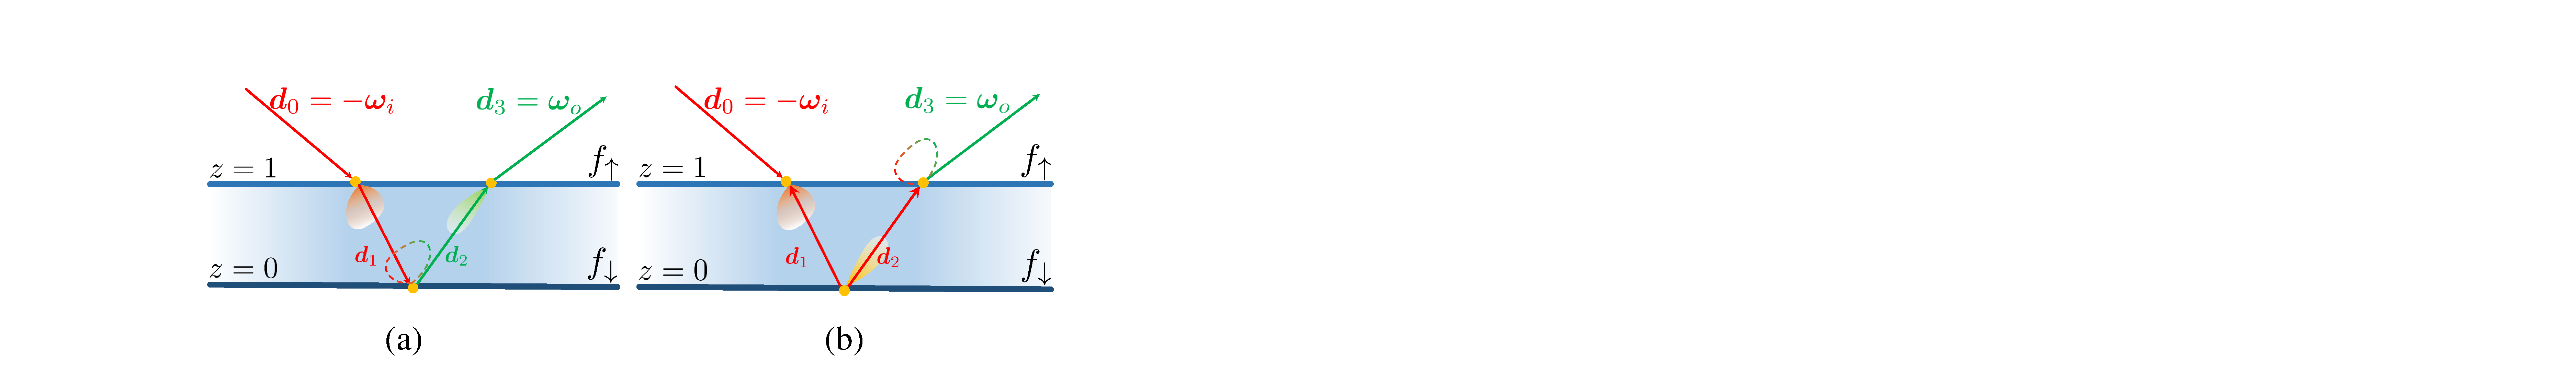
\includegraphics[width=0.67\textwidth]{layeredbsdf/illustration/unidir.pdf}
	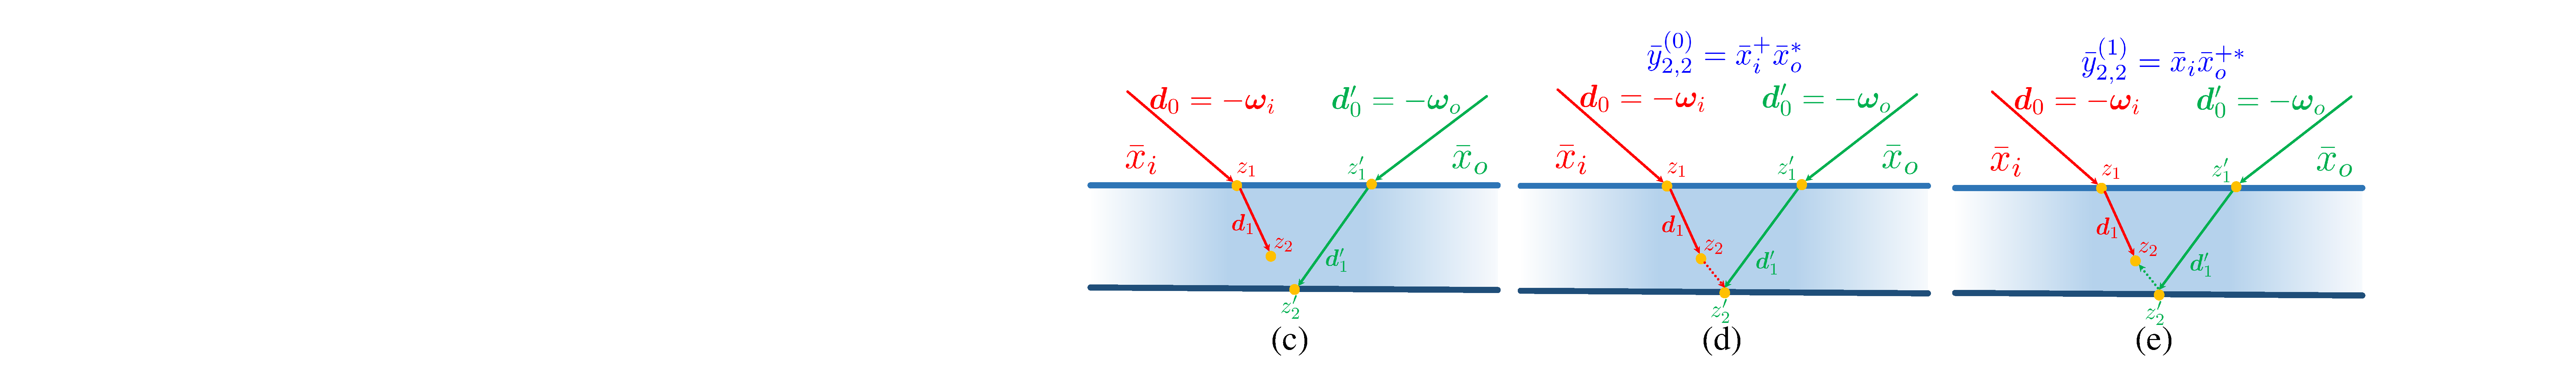
\includegraphics[width=\textwidth]{layeredbsdf/illustration/bidir.pdf}
	\caption[Our Monte Carlo estimators]{\label{fig:layeredbsdf:mc_estimators}
		\textbf{Our Monte Carlo estimators} for BSDF values.
		\textbf{(ab)} Unidirectional estimator uses two path sampling strategies for ``shading'' a vertex on the bottom layer:
		(a) sampling the BSDF $f_\uparrow$ of the top interface and connecting at the bottom (next event estimation); or (b) sampling $\bmd_2$ using $f_\downarrow$ and connecting at the top (path continuation). These strategies are combined using local MIS. \textbf{(cde)} Bidirectional estimator: (c) Two subpaths with initial directions $\bmomegai$ and $\bmomegao$. (de) Two full light paths constructed by sampling an additional direction from each sub-path.
	}
\end{figure}


Previous work on next-event estimation in scattering volumes through refractive interfaces \cite{walter2009single,koerner2016subdivision} is related to our scheme, but focuses on arbitrary geometries, which is not necessary in the flat layer setting.

Extending this NEE scheme to cross multiple layer interfaces is somewhat tedious to implement, as care must be taken not to double-count light paths. We instead use the recursive nesting approach to multiple layers (\S\ref{subsec:multi_layer}) when using the unidirectional estimator, which handles these issues automatically.


\subsubsection{Bidirectional simulation}
\label{sssec:ours_bidir}

Although our unidirectional solution works well in many cases, we introduce a new bidirectional approach that performs even better.
Our approach is conceptually similar to bidirectional path tracing (BDPT) but is technically different in several ways due to our position-free path formulation.

Given the incoming and outgoing directions $\omegain$ and $\omegaout$, consider two light transport paths, generated from the light and camera, respectively.
\begin{equation}
\begin{aligned}
\bar{x}_i &= (\bd_0, z_1, \bd_1, \ldots, z_s) \\
\bar{x}_o &= (\bd'_0, z'_1, \bd'_1, \ldots, z_t'),
\end{aligned}
\end{equation}
where $\bd_0 = -\omegain$ and $\bd'_0 = -\omegaout$ (Figure \ref{fig:layeredbsdf:mc_estimators}-c).
Now we can construct a full light path $\bar{y}_{s, t}$ connecting the $s$-th vertex in $\bar{x}_i$ and the $t$-th vertex in $\bar{x}_o$ (assuming the connection between $z_s$ and $z'_t$ does not cross any layer boundary):
\begin{equation}
\bar{y}_{s, t} = (\bd_0, \ldots, z_{s - 1}, \bd_{s - 1}, z_s, \tilde{\bd}, z'_t, -\bd'_{t - 1}, z'_{t - 1}, \ldots, -\bd'_0).
\end{equation}
Unlike traditional BDPT, where the connection term between two given subpaths endpoints is fixed, there exists infinitely many valid directions $\tilde{\bd}$ connecting $z_s$ and $z'_t$ in our case, which gives us freedom to importance-sample the direction. In practice, we choose $\tilde{\bd}$ in two ways by sampling additional directions $\bd_s$ and $\bd'_t$ by extending the two subpaths with an extra importance sampling step. We set $\tilde{\bd}$ to $\bd_s$ and $-\bd'_t$ respectively. This yields two light paths $\bar{y}^{(0)}_{s, t}$ and $\bar{y}^{(1)}_{s, t}$ (Figure \ref{fig:layeredbsdf:mc_estimators}-de), thus providing two samples of the path integral.
Denote the extended subpaths by
\begin{align}
\bar{x}_i^+ &:= (\bd_0, z_1, \bd_1, \ldots, z_s, \bd_s),\\
\bar{x}_o^+ &:= (\bd'_0, z'_1, \bd'_1, \ldots, z'_t, \bd'_t),
\end{align}
and let $\bar{x}^*$ denote the adjoint (reversed) version of a light path $\bar{x}$, e.g., \\$\bar{x}_o^{+*} = (-\bd'_t, z'_t, -\bd'_{t - 1}, \ldots, z'_1, -\bd'_0)$.

Let $v(z, \bom, \bom')$ and $s(z, z', \bom)$ be the vertex and segment contributions defined in eqs. \eqref{eqn:vtx_contrib} and \eqref{eqn:seg_contrib}.
We can easily verify that
\begin{align}
f(\bar{y}_{s,t}^{(0)}) &= f(\bar{x}_i^+) \, f(\bar{x}_o^*) \, s(z_s, z'_t, \bd_s) \, v(z'_t, -\bd_s, -\bd'_{t - 1}),\\
f(\bar{y}_{s,t}^{(1)}) &= f(\bar{x}_i) \, f(\bar{x}_o^{+*}) \, v(z_s, -\bd_{s - 1}, -\bd'_t) \, s(z_s, z'_t, -\bd'_t).
\end{align}
It follows that the two Monte Carlo estimates will be:
\begin{align}
\label{eqn:bidir_estimate_i}
\frac{f(\bar{y}^{(0)}_{s, t})}{p(\bar{y}^{(0)}_{s, t})} &=
\frac{f(\bar{x}_i^+)}{p(\bar{x}_i^+)}
\frac{f(\bar{x}_o^*)}{p(\bar{x}_o)}
\, s(z_s, z'_t, \bd_s) \, v(z'_t, -\bd_s, -\bd'_{t - 1})\\
%
\label{eqn:bidir_estimate_j}
\frac{f(\bar{y}^{(1)}_{s, t})}{p(\bar{y}^{(1)}_{s, t})} &=
\frac{f(\bar{x}_i)}{p(\bar{x}_i)}
\frac{f(\bar{x}_o^{+*})}{p(\bar{x}_o^+)}
\, v(z_s, \bd_{s - 1}, \bd'_t) \, s(z_s, z'_t, -\bd'_t),
\end{align}
Note that in general $f(\bar x_o) \neq f(\bar x_o^*)$ and $f(\bar x_o^+) \neq f(\bar x_o^{+*})$ due to non-reciprocal operations such as shading normals; care must be taken to compute correct throughputs of light subpaths, as detailed in Chapter 5 of Veach \cite{veach1997robust}.

The above discussion assumed a single light and single camera subpath. In practice, we combine all prefixes of the sampled subpaths. In particular, we sample subpaths of length $n_i$ and $n_o$ from the light and camera respectively (the lengths are chosen through Russian roulette):
\begin{equation}
\begin{aligned}
\bar{x}_i &= (\bd_0, z_1, \bd_1, \ldots, z_{n_i}, \bd_{n_i}),\\
\bar{x}_o &= (\bd'_0, z'_1, \bd'_1, \ldots, z'_{n_o}, \bd'_{n_o}).
\end{aligned}
\end{equation}
For all $s$ and $t$ combinations, Eqs. \eqref{eqn:bidir_estimate_i} and \eqref{eqn:bidir_estimate_j} provide $2 n_i n_o$ estimators of $f_l(\omegain, \omegaout)$.
Combining them using MIS gives us our bidirectional estimator for paths of length 2 or more vertices. We handle single vertex paths separately. The details of MIS weighting are discussed in the supplementary document.


\subsection{Pdf estimation}
\label{subsec:ours_pdf}

Another important operation for practical BSDF models is to evaluate the probability density for sampling provided incoming and outgoing directions.
That is, to evaluate $p(\omegaout \;|\; \omegain)$, the probability density of $\omegaout$ given $\omegain$ (assuming that the sampling process draws $\omegaout$ and fixes $\omegain$).
This operator is used for weight computation in multiple importance sampling (using balance or power heuristics), a crucial technique for generating low-noise results using scene-level Monte Carlo rendering techniques. Note that this pdf is in the solid angle measure; it is a marginal pdf distinct from the path pdf $p(\bar x)$.

Although $p(\omegaout \;|\; \omegain)$ is usually easily available for traditional analytical BSDFs, no closed-form pdf exists in our case. Instead, the pdf evaluation has comparable form to the BSDF evaluation itself. It can be expressed using another position-free path integral:
\begin{equation}
\label{eqn:ours_pdf}
p(\omegaout \;|\; \omegain) = \int_{\Omega(\omegain, \omegaout)} \mathcal{P}(\bar{x}) \intd\mu(\bar{x}),
\end{equation}
where
\begin{equation}
\mathcal{P}(\bar{x}) := \left(\prod_{j = 1}^k p(\bd_j \;|\; z_j, \bd_{j - 1})\right) \left(\prod_{j = 1}^{k - 1} p(z_{j + 1} \;|\; z_j, \bd_{j - 1})\right),
\end{equation}
with $k$ denoting the number of vertices in $\bar{x}$. Note that $\bd_k = \omegaout$.

We introduce two nondeterministic methods, an unbiased and a fast approximate approach, to estimate $p(\omegaout \;|\; \omegain)$.
These operations are not used in standard Monte Carlo light transport and are new, to our knowledge.
In practice, the approximate approach can be used when exact estimations are unnecessary (as is the case for a global path tracer with MIS, which we use for our results).
Note that the estimated $p(\omegaout \;|\; \omegain)$ is only ever used for MIS weight computation.
We never use approximate path pdfs for Monte Carlo estimates, as this would introduce bias.
Our BSDF value estimators directly return path throughput with accurate pdf factored in.

\subsubsection{Unbiased pdf estimation}
\label{sssec:ours_pdf_unbiased}

Both our unidirectional and bidirectional Monte Carlo estimators introduced in \S\ref{subsec:ours_eval} can be adapted to estimate the path integral in Eq. \eqref{eqn:ours_pdf} in an unbiased manner.
For instance, the estimators given by Eqs. \eqref{eqn:bidir_estimate_i} and \eqref{eqn:bidir_estimate_j} simply require a replacement of $f$ by $\mathcal P$, and become:
\begin{align}
	\label{eqn:bidir_pdf_i}
	\frac{\mathcal{P}(\bar{y}^{(0)}_{s, t})}{p(\bar{y}^{(0)}_{s, t})} &= \frac{\mathcal{P}(\bar{x}_o^*)}{p(\bar{x}_o)}
	 p( \bd_s \;|\; z'_t, -\bd'_{t - 1}) \, p(z'_t \;|\; z_s, \bd_s),\\
	\label{eqn:bidir_pdf_j}
	\frac{\mathcal{P}(\bar{y}^{(1)}_{s, t})}{p(\bar{y}^{(1)}_{s, t})} &= \frac{\mathcal{P}(\bar{x}_o^{+*})}{p(\bar{x}_o^+)}
	 p( \bd'_t \;|\; z_s, \bd_{s - 1}) \, p(z_s \;|\; z'_t, \bd'_t ).
\end{align}
Note that some cancellation occurs because $p(x_i) = \mathcal P(x_i)$, but in general $p(x_o) \neq \mathcal P(x_o^*)$.

When jointly estimating the path integrals for the BSDF value \eqref{eq:pathintegral} and the conditional probability \eqref{eqn:ours_pdf}, the light transport paths $\bar{x}$ need to be sampled \emph{independently} to ensure unbiasedness.
Please refer to the supplemental document for a proof.

\subsubsection{Approximate pdf estimation}
\label{sssec:ours_pdf_approx}
%
Although the adapted estimators defined in \ref{sssec:ours_pdf_unbiased} provide unbiased pdf estimations, they introduce computational overhead comparable to the BSDF evaluation itself.
Thus, for applications where unbiased pdfs are unnecessary, we introduce an approximation to accelerate the pdf estimation process. The key idea is to only consider short paths reflecting/refracting from interfaces, as these events have the largest effect on the pdf lobe shape, and add a constant (Lambertian) term to approximate the effect of volume scattering and longer paths.

In practice, we run Monte Carlo simulation on a simplified layer configuration where all volumetric media are removed.
We further limit the maximal number of vertices on the light paths to $(2L + 1)$ when $\omegain \cdot \omegaout > 0$ (i.e., $f_l(\omegain, \omegaout)$ captures reflection) and $(L + 1)$ when $\omegain \cdot \omegaout < 0$ (i.e., $f_l(\omegain, \omegaout)$ captures transmission) where $L$ denotes the number of layers.
Lastly, we add a small constant term to the estimation result. The exact scaling of this term is not important for MIS weighting (as it will be overwhelmed by the pdfs of sharply peaked lobes) and we found setting it to 0.1 works well.

\begin{figure}[h]
	\centering
	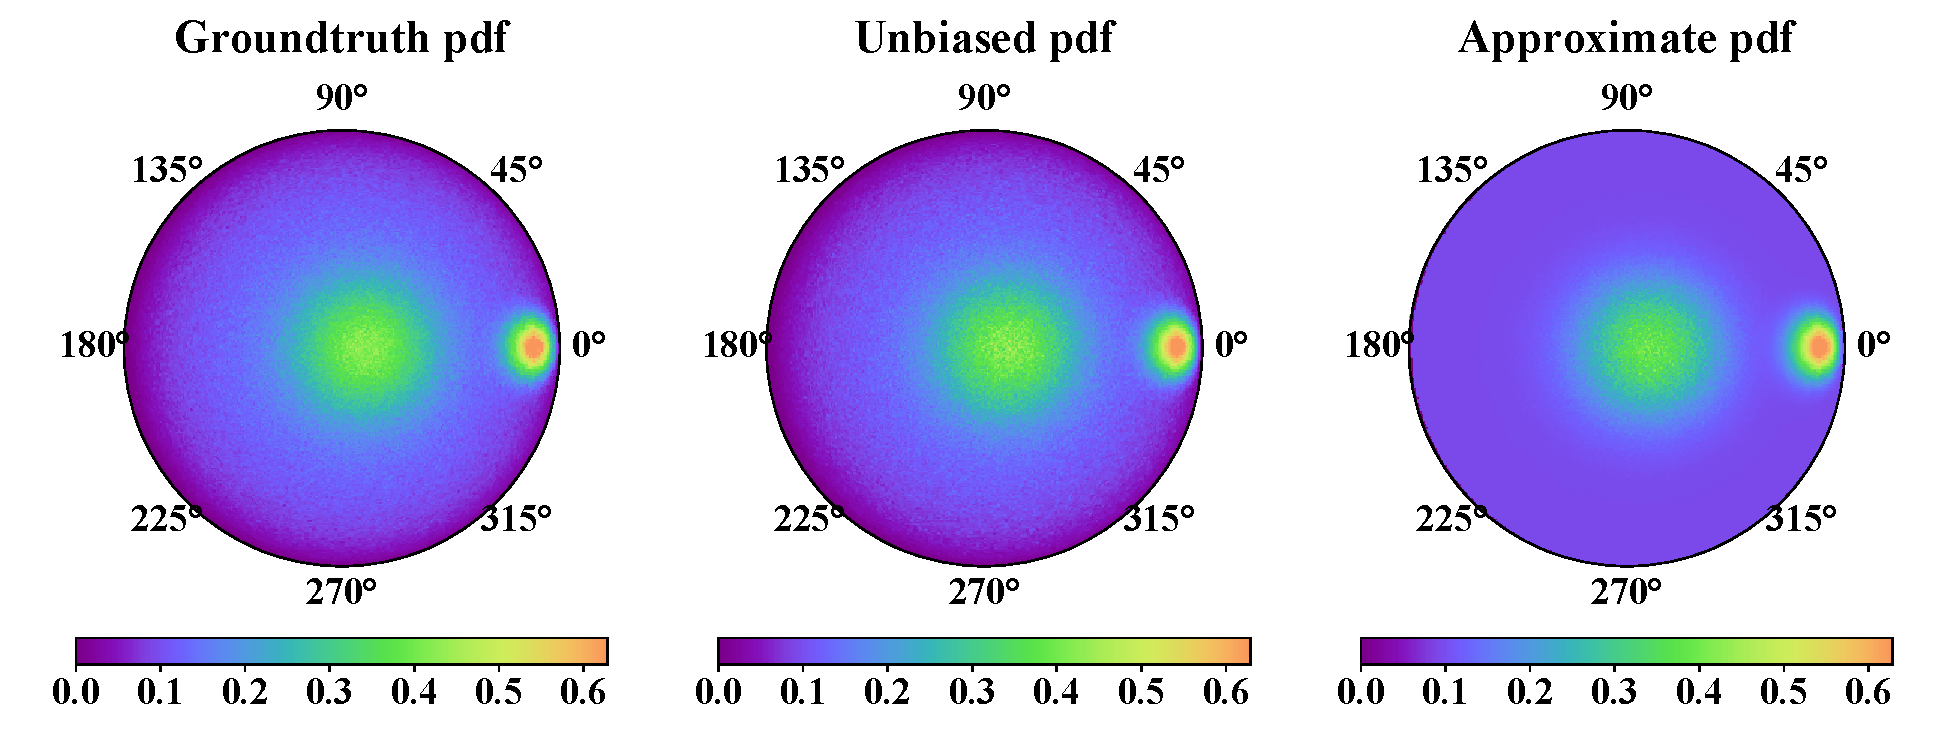
\includegraphics[width=\textwidth]{layeredbsdf/validations/lobe_pdf/pdf.pdf}
	\caption[Validation of our pdf estimates]{\label{fig:layeredbsdf:validate_pdf}
		\textbf{Validation of our pdf estimates.} The visualization applies a $\log(1+x)$ map for better shape perception. \textbf{Left:} Ground truth by sampling and binning. \textbf{Middle:} Using the unbiased pdf from \S\ref{sssec:ours_pdf_unbiased}. \textbf{Right:} Using the approximate pdf from \S\ref{sssec:ours_pdf_approx} matches the shape of the most important features and approximates longer paths and volume scattering as diffuse.
	}
\end{figure}


See Figure \ref{fig:layeredbsdf:validate_pdf} for validation of the above pdf approaches against ground truth, and Figure \ref{fig:layeredbsdf:mis} for a comparison between renderings using the unbiased and approximated pdf estimation results. 
All the other results in our paper are using approximated PDF for MIS. Unbiased PDF is much slower, because it requires long light paths, and has to be computed twice per shading event.

\begin{figure}[h]
	\centering
	\setlength{\resLen}{2.1in}
	\addtolength{\tabcolsep}{-4pt}
	\begin{tabular}{ccc}
		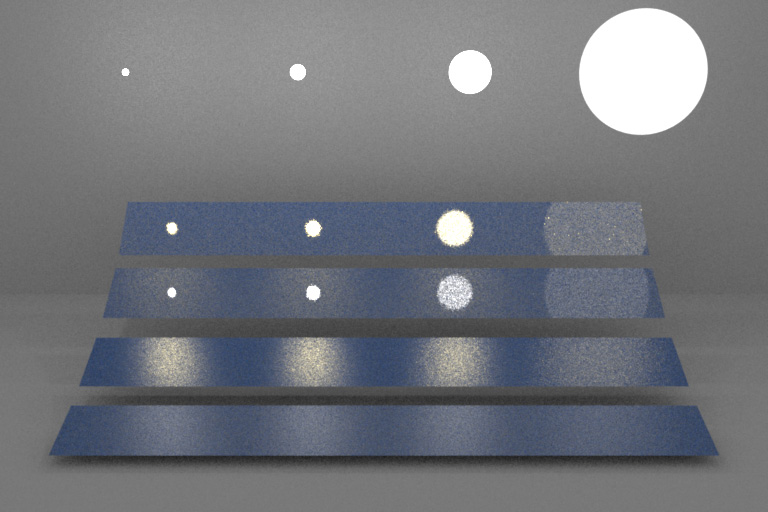
\includegraphics[width=\resLen]{layeredbsdf/validations/mis/mi_acr_64spp_14min.jpg} & 
		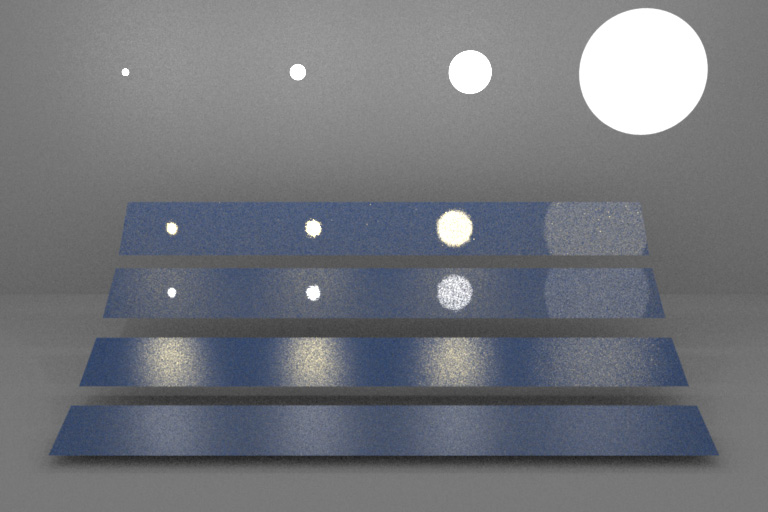
\includegraphics[width=\resLen]{layeredbsdf/validations/mis/mi_trt_64spp_4_1min.jpg} & 
		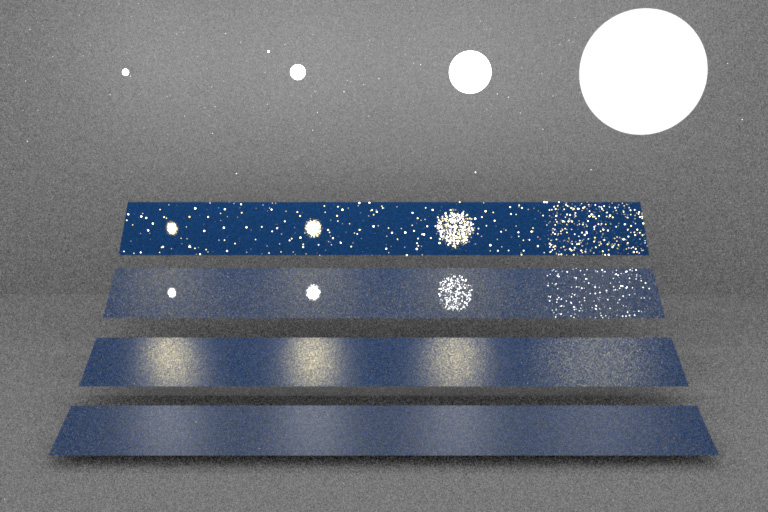
\includegraphics[width=\resLen]{layeredbsdf/validations/mis/mi_noMIS_80spp_4_2min.jpg} \\
		MIS + unbiased pdf (14 min) &
		MIS + approx. pdf (4 min) &
		no MIS (4 min) \\ 
	\end{tabular}
	\caption[Multiple importance sampling]{\label{fig:layeredbsdf:mis}
		\textbf{Multiple importance sampling} using our BSDFs.
		The slabs in this figure use a layered material with rough dielectric on the top, rough gold conductor on the bottom, and blueish homogeneous scattering medium in between.
		\textbf{Left:} Using the unbiased pdf for MIS in a traditional global path tracer. \textbf{Middle:} Using the approximate pdf is faster and gives equivalent quality. \textbf{Right:} Using no MIS is clearly inferior.
	}
\end{figure}



